% \documentclass[a4paper, onecolumn, 11pt]{IEEEtran}
\documentclass[journal,12pt,onecolumn,draftclsnofoot]{IEEEtran}
% \documentclass[a4paper, onecolumn, 12pt, doublespacing]{IEEEtran}

\usepackage[noadjust]{cite}
\usepackage{epsfig}
\usepackage{amsmath}
\usepackage{amssymb}
\usepackage{color}
\usepackage{comment}
\usepackage{subcaption}
\usepackage{float}

\input{Symbol_Shortcut.tex} % Symbols defined by Victor


\newtheorem{theorem}{\bf Theorem}		% by Victor
\newtheorem{corollary}{\bf Corollary}	% by Victor
\newtheorem{definition}{\bf Definition}	% by Victor

\pagenumbering{arabic}
% \pagestyle{empty}

\makeatletter
\def\ifundefined{\@ifundefined}
\makeatother

\setlength{\parskip}{0ex}

\begin{document}

    \title{ ADSP TFA \& ASP Report }
    \author{312510197 Zhao-Jie, Luo\\
        \small{Jun. 17, 2024}}

    \markboth{ ADSP TFA \& ASP Report}{}

    \maketitle


    \noindent \textbf{Question 2.1}
    % \section{Introduction}
        \begin{figure}[H]
            \centering
            \begin{subfigure}[b]{0.45\linewidth}
                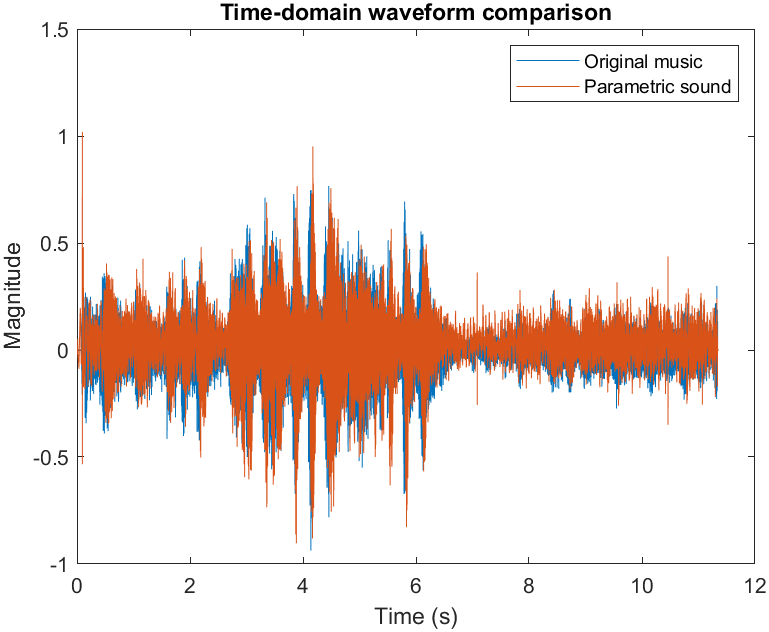
\includegraphics[width=\linewidth]{figures/time-domain waveform comparison.png}
                \caption{time-domain waveform comparison}
                \label{fig:time-domain waveform comparison}
            \end{subfigure}
            \begin{subfigure}[b]{0.45\linewidth}
                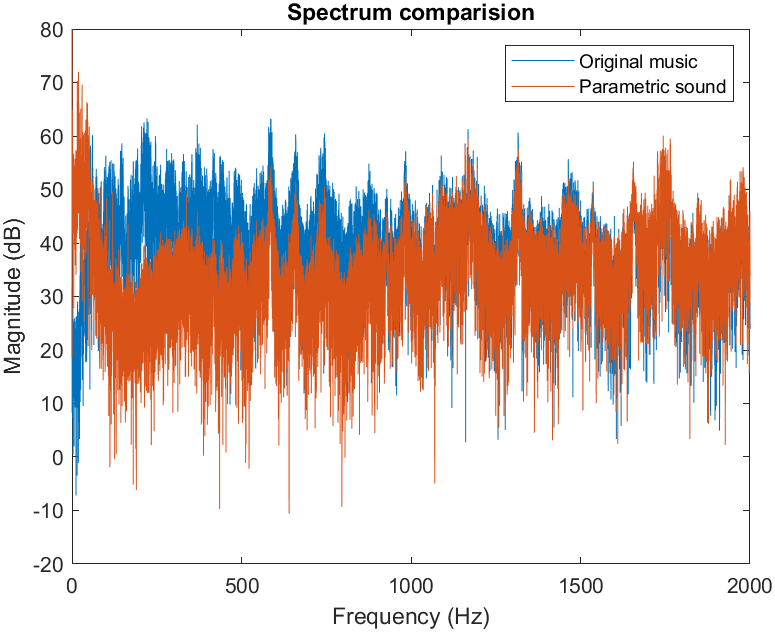
\includegraphics[width=\linewidth]{figures/spectrum comparison.png}
                \caption[short]{spectrum comparison}
                \label{fig:spectrum comparison}
            \end{subfigure}
            \caption{Comparison between 2 voices}
            % \label{fig:four_images}
        \end{figure}

        The left figure above (\ref{fig:time-domain waveform comparison}) shows a time-domain waveform comparison between the original sound and the parametric sound. 
        As illustrated, the two waveforms appear almost identical, making it challenging to distinguish or describe any differences between them.

        In contrast, the right figure above (\ref{fig:spectrum comparison}) presents a spectral comparison of the original sound and the parametric sound. 
        It is evident that there is a significant difference in the low-frequency range, where the two sounds are nearly opposite to each other. 
        However, in the high-frequency range, the similarities between them become more apparent.
        \newpage

    \noindent \textbf{Question 2.2}
        \begin{figure}[H]
            \centering
                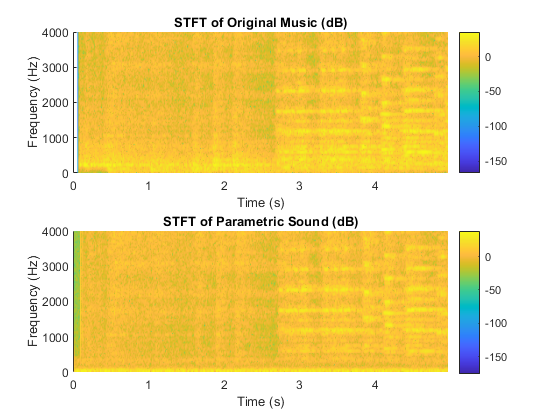
\includegraphics[width=0.7\linewidth]{figures/STFT result 1024.png}
            \caption{STFT of the original and parametric sounds with window length 1024}
            \label{fig:STFT result 1024}
        \end{figure}
        \begin{figure}[H]
            \centering
                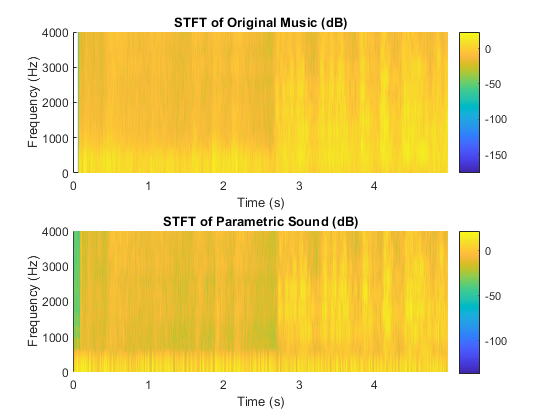
\includegraphics[width=0.7\linewidth]{figures/STFT result 128.png}
            \caption{STFT of the original and parametric sounds with window length 128}
            \label{fig:STFT result 128}
        \end{figure}

        \begin{figure}[H]
            \centering
                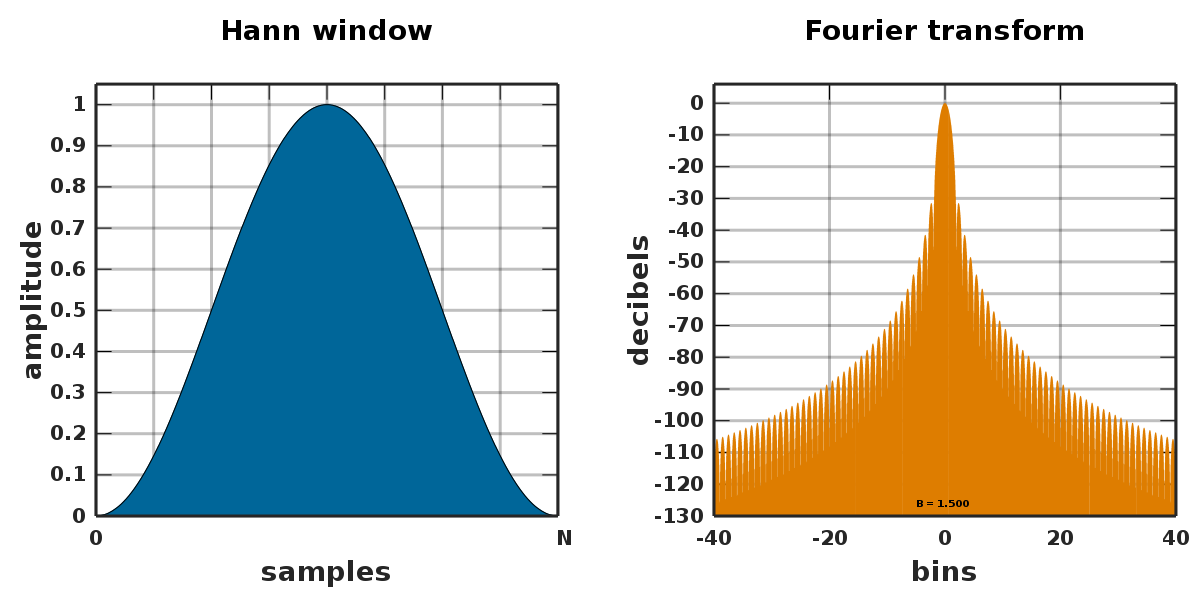
\includegraphics[width=0.7\linewidth]{figures/hann window.png}
            \caption{Hann function (left), and its frequency response (right) (source: wiki)}
            \label{fig:hann window}
        \end{figure}

        \begin{table}[H]
        \centering
        \begin{tabular}{|c|c|c|}
            \hline 
            setting & variable & value \\ \hline \hline
            window size for STFT & w\_len & 1024 \& 128 \\ \hline
            Windowing function & win & Hann window \\ \hline
            FFT length for STFT & fft\_len & 2048 \\ \hline
            Overlapping window length between two STFT analses & OverlapLength & 512 \& 64 \\ \hline
        \end{tabular} 
        \caption[short]{The settings of STFT} 
        \label{table}
        \end{table}

        The table above (\ref{table}) details the settings used for STFT analysis, including (1) window size, (2) windowing function, (3) FFT length, and (4) overlapping window length.

        I used two different window lengths, 1024 and 128, to observe varying frequency-time relationships. In Figure (\ref{fig:STFT result 1024}), 
        which employs a window length of 1024, a notable difference in low frequencies is apparent regardless of time. 
        Conversely, Figure (\ref{fig:STFT result 128}), using a window length of 128, exhibits a similar phenomenon, although withjaggedness in the low frequencies. 
        However, in the high frequencies, both figures show nearly identical results.

        Comparing the two figures using window lengths of 1024 and 128, it is evident that the first figure exhibits higher frequency-domain resolution but 
        lower time-domain resolution compared to the second figure. This observation aligns with our initial findings.
        \newpage
        
    \noindent \textbf{Question 2.3}

        Observe the STFT figures of the original and parametric sounds; there is a significant difference between them. 
        To address this, I used a Butterworth band-pass filter to first filter out the low-frequency components of the parametric sound. 
        Then, I linearly combined the filtered version with the original parametric sound. This process made the parametric sound more similar to the original one.

        The figure below shows the STFT of the original sound compared to the improved version. 
        It can be seen that the improved version is more similar to the original sound than the parametric version.

        \begin{figure}[H]
            \centering
                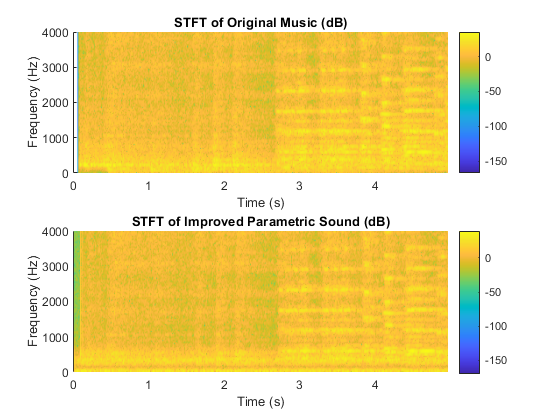
\includegraphics[width=0.7\linewidth]{figures/STFT result improved.png}
            \caption{STFT of the original and parametric sounds with window length 1024}
            \label{fig:STFT result 1024}
        \end{figure}

        

    % \bibstyle{abbrv}
    % \begin{thebibliography}{1}
    % \bibitem{Carrson}
    %     C. C. Fung, and D. Ivakhnenkov, "Model-Driven Neural Network Based MIMO Channel Estimator".
    % \bibitem{Eisen2019conf}
    %     M. Eisen and A. Ribeiro, ``Large scale wireless power allocation with graph neural networks,'' \emph{Proc. of the 2019 IEEE 20th Workshop on Signal Processing Advances in Wireless Communications (SPAWC)}, pp. 1-5, 2019.
    % \bibitem{Eisen2019journal}
    %     M. Eisen, C. Zhang, L.F.O. Chamon, D.D. Lee and A. Ribeiro, ``Learning optimal power allocations in wireless systems,'' \emph{IEEE Trans. on Signal Processing}, vol. 67(10), pp. 2775-2790, May 2019.
    % \bibitem{Eisen2020}
    %     M. Eisen and A. Ribeiro, ``Optimal wireless resource allocation with random edge graph neural networks,'' \emph{IEEE Trans. on Signal Processing}, vol. 68, pp. 2977-2991, 2020.
    % \bibitem{Naderi2022}    
    %     N. NaderiAlizadeh, M. Eisen and A. Ribeiro, ``State-Augmented learnable algorithms for resource management in wireless networks,'' \emph{IEEE Trans. on Signal Processing}, vol. 70, pp. 5898-5912, Dec. 2022.
    % \bibitem{Naderi2023}    
    %     N. NaderiAlizadeh, M. Eisen and A. Ribeiro, ``Learning resilient radio resource management policies with graph neural networks,'' \emph{IEEE Trans. on Signal Processing}, volo. 71, pp. 995-1009, Mar. 2023.
    % \end{thebibliography}

\end{document}




